\chapter{Random Groups: Class Groups, Selmer Groups and Ranks}\label{ch:06c}

In 1801 Gauss tabulated class numbers of binary quadratic forms and noticed regularities that he could not explain, among them that the determinants he called irregular, those whose principal genus (the subgroup of squares in the form class group) is not cyclic, are comparatively rare. Gauss had no notion of a random group, and the probabilistic reading of his tables had to wait until 1983, when Henri Cohen and Hendrik Lenstra proposed that class groups of quadratic fields behave like finite abelian groups drawn at random, each group $G$ weighted in proportion to $1/|\operatorname{Aut}G|$ \cite{cohenlenstra1984}. The same principle now organises a large part of arithmetic statistics. Selmer groups and Shafarevich Tate groups of elliptic curves, and with them the ranks of Mordell Weil groups, are modelled by intersections of random isotropic subspaces and by cokernels of random alternating matrices, and several of their predictions are now theorems. This chapter develops the random group models, proves their basic properties, records what is known, and compares the predictions with data computed for this book.

\section{Why random groups}\label{sec:06cwhy}

The previous chapters studied measures on compact groups: Frobenius conjugacy classes in $\SU(2)$ or $\USp(4)$, and eigenvalues of Haar random matrices in large classical groups. Those measures govern the \emph{analytic} side of the Langlands programme, the Satake parameters and the zeros of $L$ functions. The \emph{arithmetic} side, the groups that $L$ functions are conjectured to measure, has its own random models, and the measures that appear are again Haar measures, now on profinite objects such as $M_n(\Z_p)$.

Two instances anchor the connection with the Langlands programme.

The first is class field theory, the case $\GL_1$ of the programme. For a number field $K$ the Artin map identifies the class group $\mathrm{Cl}(K)$ with the Galois group of the Hilbert class field, the maximal abelian extension unramified at all places. Characters of $\mathrm{Cl}(K)$ are exactly the finite order automorphic representations of $\GL_1(\A_K)$ that are unramified at every finite place and trivial at the infinite places, and their Hecke $L$ functions factor the Dedekind zeta function of the Hilbert class field. A random model for class groups is therefore a random model for the unramified automorphic spectrum of $\GL_1$ over $K$, and questions about the $p$ part of $\mathrm{Cl}(K)$ are questions about cyclic unramified extensions of degree $p$, that is, about number fields of a prescribed type. The theorem of Davenport and Heilbronn in Section~\ref{sec:06ctheorems} is proved by counting cubic fields.

The second is the conjecture of Birch and Swinnerton Dyer \cite{bsd1965}. For an elliptic curve $E/\Q$, modularity \cite{wiles1995,taylorwiles1995,bcdt2001} attaches to $E$ a holomorphic newform of weight $2$, so $L(s,E)$ is an automorphic $L$ function of $\GL_2$, entire, with a functional equation and a root number $w(E) = \pm1$. The conjecture predicts that the order of vanishing at the centre equals the rank $r(E)$ of $E(\Q)$, and that the leading coefficient involves the order of the Shafarevich Tate group $\mathrm{Sha}(E)$. Selmer groups sit between the two: they are finite, computable, and bound the rank from above. A random model for Selmer groups and $\mathrm{Sha}$ is therefore a random model for the arithmetic data that the central behaviour of an automorphic $L$ function is conjectured to encode.

The guiding heuristic, in both settings, is that an arithmetic group should be distributed like a random object chosen with probability inversely proportional to its number of symmetries, after the constraints imposed by the arithmetic (units, duality pairings, roots of unity) have been accounted for. When the constraints are correctly identified the models agree with the theorems and with the data; when they are missed the models fail in instructive ways, as Malle discovered for class groups in the presence of roots of unity \cite{malle2008}.

\section{The Cohen Lenstra measure}\label{sec:06ccl}

Throughout, $p$ is a prime and $G$ runs through isomorphism classes of finite abelian $p$ groups. Write
\[
\eta_n(p) = \prod_{k=1}^n(1-p^{-k}),\qquad \eta_\infty(p) = \prod_{k=1}^\infty(1-p^{-k}),
\]
so that $\eta_\infty(2) = 0.288788$, $\eta_\infty(3) = 0.560126$, $\eta_\infty(5) = 0.760333$ and $\eta_\infty(7) = 0.836795$. The $p$ rank of $G$ is $\operatorname{rk}_pG = \dim_{\mathbb{F}_p}G/pG = \dim_{\mathbb{F}_p}G[p]$.

\begin{definition}\label{def:06ccl}
The Cohen Lenstra measure on finite abelian $p$ groups is
\[
\mu_{\mathrm{CL}}(G) = \frac{\eta_\infty(p)}{|\operatorname{Aut}G|}.
\]
\end{definition}

The cyclic group $\Z/p^2$ has $p(p-1)$ automorphisms while $(\Z/p)^2$ has $(p^2-1)(p^2-p)$, so among groups of order $p^2$ the measure prefers the cyclic one by the factor $p^2-1$, in agreement with Gauss's observation that irregular determinants, those with noncyclic principal genus, are rare. That $\mu_{\mathrm{CL}}$ is a probability measure is equivalent to the identity
\begin{equation}\label{eq:06chall}
\sum_G\frac{1}{|\operatorname{Aut}G|} = \prod_{k=1}^\infty(1-p^{-k})^{-1},
\end{equation}
which goes back to P.~Hall \cite{hall1938}. We prove it, together with the random matrix model of Friedman and Washington \cite{friedmanwashington1989}, in a single argument.\index{Cohen Lenstra measure}\index{Hall's identity}

\subsection{Cokernels of random $p$ adic matrices}

Let $A_n$ be a random matrix in $M_n(\Z_p)$ drawn from Haar probability measure, so that its entries are independent and uniform on $\Z_p$. The set $\{\det A = 0\}$ is a proper analytic subset and has Haar measure zero, so almost surely $\det A_n\ne0$ and $\operatorname{cok}A_n = \Z_p^n/A_n\Z_p^n$ is a finite abelian $p$ group of order $p^{v_p(\det A_n)}$. For a finite abelian $p$ group $B$ of $p$ rank $r$, a homomorphism $\Z_p^n\to B$ is surjective if and only if its reduction $\mathbb{F}_p^n\to B/pB\cong\mathbb{F}_p^r$ is, so
\begin{equation}\label{eq:06csur}
|\operatorname{Sur}(\Z_p^n,B)| = |B|^n\prod_{j=0}^{r-1}(1-p^{j-n}) = |B|^n\prod_{k=n-r+1}^{n}(1-p^{-k}),
\end{equation}
an empty product being $1$ (and the count is $0$ when $r>n$).

\begin{theorem}[Hall; Friedman and Washington]\label{thm:06cfw}
For every finite abelian $p$ group $G$ of $p$ rank $r\le n$,
\[
\Prob(\operatorname{cok}A_n\cong G) = \frac{1}{|\operatorname{Aut}G|}\,\eta_n(p)\prod_{k=n-r+1}^n(1-p^{-k}),
\]
and as $n\to\infty$ this tends to $\mu_{\mathrm{CL}}(G)$. Moreover $\mu_{\mathrm{CL}}$ is a probability measure, that is, Hall's identity \eqref{eq:06chall} holds, and $\operatorname{cok}A_n$ converges in total variation to $\mu_{\mathrm{CL}}$.
\end{theorem}

\begin{proof}
A finite module $C$ is isomorphic to $G$ if and only if there is a surjection $\varphi:\Z_p^n\to G$ with kernel $A_n\Z_p^n$, and when $C = \operatorname{cok}A_n\cong G$ the number of such $\varphi$ is exactly $|\operatorname{Aut}G|$, since any two differ by an automorphism of $G$. Hence
\[
\Prob(\operatorname{cok}A_n\cong G) = \frac{1}{|\operatorname{Aut}G|}\sum_{\varphi\in\operatorname{Sur}(\Z_p^n,G)}\Prob\bigl(A_n\Z_p^n = \ker\varphi\bigr).
\]
Fix $\varphi$ and put $L = \ker\varphi$, a sublattice of index $|G|$. The columns of $A_n$ are independent and uniform on $\Z_p^n$, and each lies in $L$ with probability $|G|^{-1}$. Conditionally on all columns lying in $L$, they are independent and uniform on $L$; choosing a basis of $L$ we may write $A_n = MC$ with $M$ a fixed matrix whose columns are that basis and $C$ Haar distributed in $M_n(\Z_p)$. Then $A_n\Z_p^n = L$ if and only if $C\Z_p^n = \Z_p^n$, that is $C\in\GL_n(\Z_p)$, which happens if and only if $C\bmod p\in\GL_n(\mathbb{F}_p)$, with probability $|\GL_n(\mathbb{F}_p)|/p^{n^2} = \eta_n(p)$. So each $\varphi$ contributes $|G|^{-n}\eta_n(p)$, and \eqref{eq:06csur} gives the formula. As $n\to\infty$ the two products tend to $\eta_\infty(p)$ and $1$.

For the remaining statements let $P_n(G)$ denote this probability. As $\det A_n\ne0$ almost surely, $\sum_GP_n(G) = 1$ for every $n$. By Fatou's lemma $\sum_G\mu_{\mathrm{CL}}(G)\le\liminf_n\sum_GP_n(G) = 1$, so that
\[
\sum_G|\operatorname{Aut}G|^{-1}\le\eta_\infty(p)^{-1}<\infty .
\]
 Now $P_n(G)\le|\operatorname{Aut}G|^{-1}$ for all $n$ and $G$, because the two products are at most $1$; this domination is summable, and dominated convergence gives $\sum_G\mu_{\mathrm{CL}}(G) = \lim_n\sum_GP_n(G) = 1$, which is \eqref{eq:06chall}. Pointwise convergence of probability mass functions to a probability mass function implies convergence in total variation (Scheff\'e's lemma).
\end{proof}

The case $G = 0$ is worth isolating, since it is the simplest instance and the one most often used.

\begin{corollary}\label{cor:06crank0}
For Haar random $A_n\in M_n(\Z_p)$, $\Prob(\operatorname{cok}A_n = 0) = \Prob(A_n\in\GL_n(\Z_p)) = \eta_n(p)\to\eta_\infty(p)$.
\end{corollary}

\begin{proof}
The cokernel vanishes if and only if $A_n$ is invertible over $\Z_p$, if and only if $\det A_n$ is a unit, if and only if $A_n\bmod p$ is invertible. The reduction is uniform on $M_n(\mathbb{F}_p)$, and $|\GL_n(\mathbb{F}_p)| = \prod_{i=0}^{n-1}(p^n-p^i) = p^{n^2}\eta_n(p)$, counting bases column by column.
\end{proof}

The proof shows what the weight $1/|\operatorname{Aut}G|$ means probabilistically: the natural Haar measure is on presentations (surjections from a free module), and a group with many automorphisms has proportionally fewer distinct presentations. This is the same mechanism as the orbit counting behind the weight $1/|\operatorname{Aut}|$ in every mass formula of Siegel type.

\subsection{The $p$ rank law and the probability that $p$ divides the class number}

\begin{proposition}[Cohen and Lenstra]\label{prop:06cprank}
Under $\mu_{\mathrm{CL}}$,
\[
\mu_{\mathrm{CL}}(\operatorname{rk}_pG = r) = \frac{p^{-r^2}\,\eta_\infty(p)}{\prod_{k=1}^r(1-p^{-k})^2},\qquad r\ge0,
\]
and $\mu_{\mathrm{CL}}(G\ne0) = 1-\eta_\infty(p)$.
\end{proposition}

\begin{proof}
For each $n$, $\operatorname{rk}_p\operatorname{cok}A_n = \dim\operatorname{cok}(A_n\bmod p) = n-\operatorname{rank}_{\mathbb{F}_p}(A_n\bmod p)$, and $A_n\bmod p$ is uniform on $M_n(\mathbb{F}_p)$. The number of $n\times n$ matrices of rank $k$ over $\mathbb{F}_p$ is $\prod_{i=0}^{k-1}(p^n-p^i)^2/(p^k-p^i)$: choose the image, a $k$ dimensional subspace, in $\prod_{i<k}(p^n-p^i)/(p^k-p^i)$ ways, then a surjection onto it in $\prod_{i<k}(p^n-p^i)$ ways. With $k = n-r$,
\[
\frac{1}{p^{n^2}}\prod_{i=0}^{k-1}\frac{(p^n-p^i)^2}{p^k-p^i} = p^{2nk-k^2-n^2}\,\frac{\prod_{j=r+1}^n(1-p^{-j})^2}{\prod_{j=1}^{k}(1-p^{-j})},
\]
and $2nk-k^2-n^2 = -r^2$. Letting $n\to\infty$ gives $p^{-r^2}\eta_\infty^2/(\eta_r^2\eta_\infty)$. By Theorem~\ref{thm:06cfw} the laws of $\operatorname{cok}A_n$ converge in total variation to $\mu_{\mathrm{CL}}$, so the laws of the $p$ rank converge to its law under $\mu_{\mathrm{CL}}$. The last claim is the case $G=0$ of the definition.
\end{proof}

For $p=3$ the rank law is $0.5601$, $0.4201$, $0.0197$ for $r = 0,1,2$, and the Cohen Lenstra prediction for the proportion of imaginary quadratic fields with $3\mid h(D)$ is $1-\eta_\infty(3) = 0.4399$, well above the naive $1/3$.

\subsection{Moments}

For a fixed finite abelian $p$ group $B$, the number $|\operatorname{Sur}(G,B)|$ is a natural test function on groups: $|\operatorname{Sur}(G,\Z/p)| = |G[p]|-1$, since every nonzero homomorphism to $\Z/p$ is surjective and $|\operatorname{Hom}(G,\Z/p)| = |G[p]|$.

\begin{proposition}[Moments of the Cohen Lenstra measure]\label{prop:06cmoments}
For every finite abelian $p$ group $B$, $\E_{\mu_{\mathrm{CL}}}|\operatorname{Sur}(G,B)| = 1$. In particular $\E_{\mu_{\mathrm{CL}}}|G[p]| = 2$.
\end{proposition}

\begin{proof}
Let $r$ be the $p$ rank of $B$. Surjections $\operatorname{cok}A_n\to B$ correspond to surjections $\psi:\Z_p^n\to B$ with $\psi\circ A_n = 0$, and for fixed $\psi$ this event has probability $|B|^{-n}$, each column independently lying in $\ker\psi$. Hence, by \eqref{eq:06csur}, $\E|\operatorname{Sur}(\operatorname{cok}A_n,B)| = \prod_{k=n-r+1}^n(1-p^{-k})$, which is at most $1$ and tends to $1$. To pass the limit inside the expectation we use uniform integrability: $|\operatorname{Sur}(G,B)|^2\le|\operatorname{Hom}(G,B\times B)| = \sum_{B'\le B\times B}|\operatorname{Sur}(G,B')|$, so applying the bound just proved to each of the finitely many subgroups $B'$ of $B\times B$ shows that $\E|\operatorname{Sur}(\operatorname{cok}A_n,B)|^2$ is bounded in $n$. Since $\operatorname{cok}A_n$ converges in law to $\mu_{\mathrm{CL}}$ (Theorem~\ref{thm:06cfw}), the expectations converge to $\E_{\mu_{\mathrm{CL}}}|\operatorname{Sur}(G,B)|$, which is therefore $1$. The second statement is the case $B = \Z/p$.
\end{proof}

The moments characterise the measure. Ellenberg, Venkatesh and Westerland \cite{evw2016} proved that $\mu_{\mathrm{CL}}$ is the only probability measure on finite abelian $p$ groups all of whose $B$ moments equal $1$, in a robust form: random groups whose $B$ moments converge to $1$ for every $B$ converge in distribution to $\mu_{\mathrm{CL}}$. Wood \cite{wood2017} showed more generally that moments $M_B = O(|\wedge^2B|)$ determine the distribution, again robustly under limits. This moment method is the route by which most theorems in the subject are now proved: one counts surjections, which is a counting problem for number fields or for points on moduli spaces, and deduces the distribution.\index{moment method}

\subsection{The real quadratic variant}

For real quadratic fields the unit group has rank one, and Cohen and Lenstra proposed the weights
\[
\mu^+_{\mathrm{CL}}(G) = \frac{c_p^+}{|G|\,|\operatorname{Aut}G|},
\]
the constant being fixed by normalisation: $\sum_G|G|^{-1}|\operatorname{Aut}G|^{-1} = \prod_{k\ge2}(1-p^{-k})^{-1}$ (the matrix model below proves this as Theorem~\ref{thm:06cfw} proves \eqref{eq:06chall}; it is also the value at $x = 1/p$ of the generating function in the first exercise), so $c_p^+ = \eta_\infty(p)/(1-p^{-1})$. The $p$ rank law becomes
\[
\mu^+_{\mathrm{CL}}(\operatorname{rk}_pG = r) = \frac{p^{-r(r+1)}\,\eta_\infty(p)}{\prod_{k=1}^r(1-p^{-k})\prod_{k=1}^{r+1}(1-p^{-k})},
\]
the moments become $\E|\operatorname{Sur}(G,B)| = |B|^{-1}$, and in particular $\E|G[p]| = 1+p^{-1}$, equal to $\frac43$ for $p=3$. The matrix model is the cokernel of a Haar random $n\times(n+1)$ matrix over $\Z_p$, the extra column playing the role of the unit (Wood \cite{wood2019} proves universality for such $n\times(n+u)$ models). The proof of Theorem~\ref{thm:06cfw} adapts line by line: each $\varphi$ now contributes $|G|^{-n-1}\prod_{k=2}^{n+1}(1-p^{-k})$, which produces the extra factor $|G|^{-1}$. The convergence in $n$ is fast: for a uniformly random $8\times9$ matrix over $\mathbb{F}_3$ the exact probabilities of cokernel dimension $0$, $1$, $2$ already agree with the limits $0.8402$, $0.1575$, $0.0023$ to four decimal places.

\section{Theorems and conjectures for class groups}\label{sec:06ctheorems}

\begin{conjecture}[Cohen and Lenstra \cite{cohenlenstra1984}]\label{conj:06ccl}
Let $p$ be an odd prime and $G$ a finite abelian $p$ group. As $X\to\infty$, the proportion of negative fundamental discriminants $D$ with $|D|<X$ and $\mathrm{Cl}(D)[p^\infty]\cong G$ tends to $\mu_{\mathrm{CL}}(G)$, and the proportion of positive fundamental discriminants $D<X$ with $\mathrm{Cl}(D)[p^\infty]\cong G$ tends to $\mu^+_{\mathrm{CL}}(G)$.
\end{conjecture}

The prime $2$ is excluded because genus theory determines $\mathrm{Cl}(D)[2]$ from the number of prime factors of $D$. Gerth's modification treats $(2\mathrm{Cl}(D))[2^\infty]$; Fouvry and Kl\"uners \cite{fouvrykluners2007} proved the predicted distribution of the $4$ rank, and Smith \cite{smith2017} proved, in a preprint, the predicted distribution of $(2\mathrm{Cl}(D))[2^\infty]$ for imaginary quadratic fields. For odd $p$ the only proved case concerns $p = 3$, and only the first moment.

\begin{theorem}[Davenport and Heilbronn \cite{davenportheilbronn1971}]\label{thm:06cdh}
As $X\to\infty$, the average of $|\mathrm{Cl}(D)[3]|$ over fundamental discriminants $-X<D<0$ tends to $2$, and over fundamental discriminants $0<D<X$ it tends to $\frac43$.
\end{theorem}

The proof is a count of cubic fields. A cubic field $K$ of discriminant $D$ fundamental has Galois closure containing $\Q(\sqrt D)$, and by class field theory the nontrivial $3$ torsion characters of $\mathrm{Cl}(D)$, up to inversion, correspond to cubic fields of discriminant $D$. Cubic rings correspond to $\GL_2(\Z)$ orbits of integral binary cubic forms (Delone and Faddeev), so counting cubic fields by discriminant becomes counting lattice points in a fundamental domain for $\GL_2(\Z)$ acting on a four dimensional real space, followed by a sieve to maximal rings. Bhargava's parametrisations of rings of rank up to $5$ extended the method, and in particular gave the average size of the $2$ torsion in class groups of cubic fields, $\frac54$ for totally real and $\frac32$ for complex cubic fields \cite{bhargava2005}, in agreement with the Cohen and Martinet extension of the heuristic.

\begin{theorem}[Bhargava, Shankar and Tsimerman; Taniguchi and Thorne]\label{thm:06csecond}
Let $N_3^\pm(X)$ be the number of cubic fields $K$ with $0<\pm\operatorname{disc}K<X$, and put $C^+ = K^+ = 1$, $C^- = 3$, $K^- = \sqrt3$. There is $\delta>0$ such that
\[
N_3^\pm(X) = \frac{C^\pm}{12\zeta(3)}X + K^\pm\frac{4\zeta(\frac13)}{5\Gamma(\frac23)^3\zeta(\frac53)}X^{5/6} + O(X^{5/6-\delta}),
\]
and, with $D$ running over fundamental discriminants,
\begin{multline}\label{eq:06ctt}
\sum_{0<\pm D<X}|\mathrm{Cl}(D)[3]| = \frac{3+C^\pm}{\pi^2}X\\
+ K^\pm\frac{8\zeta(\frac13)}{5\Gamma(\frac23)^3}\prod_p\Bigl(1-\frac{p^{1/3}+1}{p(p+1)}\Bigr)X^{5/6} + O(X^{5/6-\delta}).
\end{multline}
\end{theorem}

The secondary term was conjectured by Roberts on the basis of numerical data and proved independently in \cite{bst2013} and \cite{taniguchithorne2013}; the formulas above are those of Taniguchi and Thorne, whose error terms are $O(X^{7/9+\epsilon})$ and $O(X^{18/23+\epsilon})$, while Bhargava, Shankar and Tsimerman obtain $O(X^{13/16+\epsilon})$ for the cubic fields. Since $\zeta(\frac13) = -0.9734$, both secondary terms are negative. The coefficient of $X^{5/6}$ in \eqref{eq:06ctt} is $-0.41478$ for $D<0$ and $-0.23947$ for $D>0$, and there are $(3/\pi^2)X+O(X^{1/2})$ fundamental discriminants of each sign up to $X$, so the mean of $|\mathrm{Cl}(D)[3]|$ over $0<-D<X$ is $2-1.365X^{-1/6}+O(X^{-1/6-\delta})$, and over $0<D<X$ it is $\frac43-0.788X^{-1/6}+O(X^{-1/6-\delta})$. In the imaginary case the correction is still $0.14$ at $X = 10^6$ and $0.014$ at $X = 10^{12}$: averages of $3$ torsion converge so slowly that no computation in the accessible range sees the limit directly.\index{secondary term}

For $p\ge5$, and for the full distribution at $p = 3$, Conjecture~\ref{conj:06ccl} is open: not even the average of $|\mathrm{Cl}(D)[5]|$ is known. The strongest evidence beyond number fields comes from function fields. For an odd prime $\ell$ and a finite abelian $\ell$ group $G$, Ellenberg, Venkatesh and Westerland \cite{evw2016} used homological stability for Hurwitz spaces to show that the upper and lower densities of imaginary quadratic extensions of $\mathbb{F}_q(t)$ whose class group has $\ell$ part isomorphic to $G$ both tend to $\mu_{\mathrm{CL}}(G)$ as $q\to\infty$ through odd prime powers prime to $\ell$ with $q\not\equiv1\pmod\ell$. The theorem is a limit in $q$ and does not by itself give the distribution for any fixed $q$; we refer to the paper and its sequels for the exact statements.

When the base field contains $p$th roots of unity the heuristics require modification. Malle \cite{malle2008} found in extensive computations that the $p$ parts of class groups of extensions of a base field containing $\mu_p$ do not follow the Cohen and Martinet predictions, and proposed corrected distributions; the correction reflects an additional pairing coming from the roots of unity, and the analogous phenomenon in function fields is explained by the Weil pairing on the Jacobian.

\subsection{Our data}\label{sec:06cdata}

We computed with PARI/GP (\texttt{quadclassunit}, whose output is guaranteed under the generalized Riemann hypothesis) the class groups of all $303963$ fundamental discriminants $D\in[-2\cdot10^6,-10^6]$ and of all $91185$ fundamental discriminants $D\in[10^5,4\cdot10^5]$. Table~\ref{tab:06cprank} and Figure~\ref{fig:06ccohenlenstra} compare the $p$ rank frequencies with Proposition~\ref{prop:06cprank} and its real analogue.

\begin{table}[ht]\centering\small
\begin{tabular}{llcccc}
\toprule
 & & $r=0$ & $r=1$ & $r=2$ & $\Prob(p\mid h)$\\
\midrule
imaginary, $p=3$ & observed & $0.5901$ & $0.3976$ & $0.0123$ & $0.4099$\\
 & Cohen Lenstra & $0.5601$ & $0.4201$ & $0.0197$ & $0.4399$\\
imaginary, $p=5$ & observed & $0.7662$ & $0.2321$ & $0.0017$ & $0.2338$\\
 & Cohen Lenstra & $0.7603$ & $0.2376$ & $0.0021$ & $0.2397$\\
imaginary, $p=7$ & observed & $0.8406$ & $0.1590$ & $0.0003$ & $0.1594$\\
 & Cohen Lenstra & $0.8368$ & $0.1627$ & $0.0005$ & $0.1632$\\
\midrule
real, $p=3$ & observed & $0.8768$ & $0.1227$ & $0.0004$ & $0.1232$\\
 & Cohen Lenstra & $0.8402$ & $0.1575$ & $0.0023$ & $0.1598$\\
real, $p=5$ & observed & $0.9603$ & $0.0397$ & $0.0000$ & $0.0397$\\
 & Cohen Lenstra & $0.9504$ & $0.0495$ & $0.0001$ & $0.0496$\\
real, $p=7$ & observed & $0.9814$ & $0.0186$ & $0.0000$ & $0.0186$\\
 & Cohen Lenstra & $0.9763$ & $0.0237$ & $0.0000$ & $0.0237$\\
\bottomrule
\end{tabular}
\caption{Distribution of the $p$ rank of class groups: $303963$ imaginary fundamental discriminants in $[-2\cdot10^6,-10^6]$ and $91185$ real ones in $[10^5,4\cdot10^5]$, against the Cohen Lenstra predictions.}\label{tab:06cprank}
\end{table}

\begin{figure}[ht]\centering
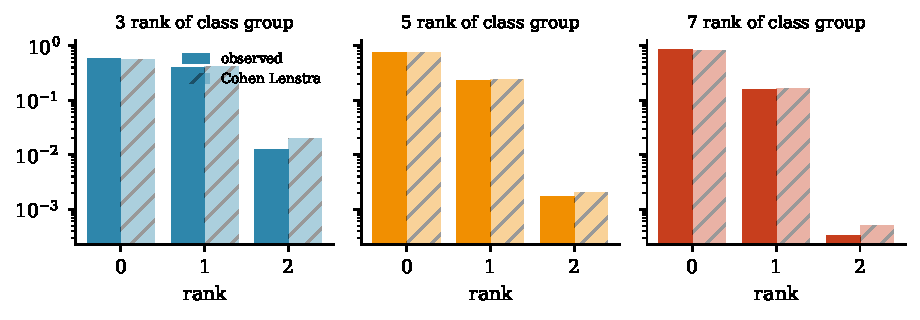
\includegraphics[width=0.92\textwidth]{figs/cohen_lenstra.pdf}
\caption{Frequencies of $3$, $5$ and $7$ ranks of class groups of imaginary quadratic fields with $10^6\le|D|\le2\cdot10^6$ (logarithmic scale), observed against the Cohen Lenstra law $p^{-r^2}\eta_\infty(p)/\prod_{k\le r}(1-p^{-k})^2$.}\label{fig:06ccohenlenstra}
\end{figure}

\begin{figure}[ht]\centering
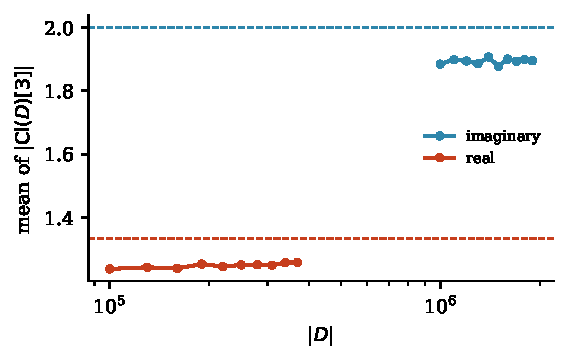
\includegraphics[width=0.7\textwidth]{figs/davenport_heilbronn.pdf}
\caption{Window means of $|\mathrm{Cl}(D)[3]|$ for imaginary ($10^6\le|D|\le2\cdot10^6$) and real ($10^5\le D\le4\cdot10^5$) quadratic fields: each range is split into ten windows with equal numbers of discriminants, and each mean is plotted at the smallest $|D|$ of its window. Dashed lines: the Davenport Heilbronn limits $2$ and $\frac43$.}\label{fig:06cdh}
\end{figure}

Three features stand out. First, the agreement improves with $p$. In the imaginary range every frequency for $p = 7$ is within $0.004$ of the prediction and every frequency for $p = 5$ within $0.006$, while for $p = 3$ the deficit in $\Prob(3\mid h)$ is $0.030$; in the real range the deficits in $\Prob(p\mid h)$ are $0.037$, $0.010$ and $0.005$ for $p = 3,5,7$. Even the small deficits are significant: in the imaginary range the binomial standard error of $\Prob(p\mid h)$ is below $0.001$, so the deficits for $p = 5$ and $p = 7$ are about $8$ and $6$ standard errors. Second, the deviations have a consistent sign: the data show too few groups with nontrivial $p$ part. Third, the mean of $|\mathrm{Cl}(D)[3]|$ is $1.8933$ in the imaginary range against the limit $2$, with window means in Figure~\ref{fig:06cdh} between $1.877$ and $1.907$ and no visible trend, and $1.2489$ in the real range against $\frac43$.

The secondary term of Theorem~\ref{thm:06csecond} accounts for the $3$ torsion deficit quantitatively. The nontrivial part of the mean, $\E|\mathrm{Cl}(D)[3]|-1$, is $0.893$ against $1$ in the imaginary range and $0.249$ against $\frac13$ in the real range, relative deficits of $0.107$ and $0.253$. Taking differences of \eqref{eq:06ctt} at the ends of our two ranges and dividing by the number of fundamental discriminants in them predicts means of $1.8933$ for $-2\cdot10^6\le D\le-10^6$ and $1.2496$ for $10^5\le D\le4\cdot10^5$, against the observed $1.8933$ and $1.2489$; with the variance of $|G[3]|$ under the Cohen Lenstra measures, the standard error of each observed mean is about $0.003$. The larger relative deficit of the real range has two sources: its discriminants are about six times smaller, which multiplies $X^{-1/6}$ by $6^{1/6} = 1.35$, and its secondary coefficient, measured against the main term of the nontrivial part ($3/\pi^2$ for $D<0$, $1/\pi^2$ for $D>0$), is larger by the factor $\sqrt3$. Across the imaginary range \eqref{eq:06ctt} predicts window means rising only from $1.887$ to $1.898$, a change comparable to the standard error $0.008$ of a single window mean, so the flat window means of Figure~\ref{fig:06cdh} are expected; across the real range it predicts a rise from $1.239$ to $1.256$, and the data go from $1.238$ to $1.259$. For $p = 5$ and $p = 7$ no secondary term is known; the smaller deficits suggest one that is smaller or decays faster. The lesson for the computational programme is that data should be compared with Cohen and Lenstra only after the secondary term is accounted for, from \eqref{eq:06ctt} where it is known and by fitting a correction $c'X^{-\theta}$ with a free exponent where it is not (Computational Problem~\ref{cp:06cclscale}).

\section{Selmer groups and the Poonen Rains model}\label{sec:06cselmer}

Let $E/\Q$ be an elliptic curve and $n\ge2$. The Kummer sequence $0\to E[n]\to E(\bar\Q)\xrightarrow{n}E(\bar\Q)\to0$ gives an injection $E(\Q)/nE(\Q)\hookrightarrow H^1(\Q,E[n])$, and similarly over every completion $\Q_v$. The $n$ Selmer group\index{Selmer group} $\operatorname{Sel}_n(E)$ is the subgroup of classes in $H^1(\Q,E[n])$ whose restriction to every $\Q_v$ lies in the image of $E(\Q_v)/nE(\Q_v)$; it is finite and effectively computable. The Shafarevich Tate group $\mathrm{Sha}(E)$\index{Shafarevich Tate group} is the group of isomorphism classes of torsors under $E$ that have a point over every completion of $\Q$, and the descent sequence reads
\begin{equation}\label{eq:06cdescent}
0\to E(\Q)/nE(\Q)\to\operatorname{Sel}_n(E)\to\mathrm{Sha}(E)[n]\to0 .
\end{equation}
When $E(\Q)[2] = 0$ we have $E(\Q)/2E(\Q)\cong(\Z/2)^{r}$, so $r(E)\le\dim_{\mathbb{F}_2}\operatorname{Sel}_2(E)$, with equality if and only if $\mathrm{Sha}(E)[2] = 0$. If $\mathrm{Sha}(E)[2^\infty]$ is finite, the Cassels Tate pairing on it is alternating and nondegenerate, so $|\mathrm{Sha}(E)[2]|$ is a square and $\dim\operatorname{Sel}_2\equiv r\pmod 2$.

\subsection{Intersections of random maximal isotropic subspaces}

Poonen and Rains \cite{poonenrains2012} proved that $\operatorname{Sel}_p(E)$ is naturally an intersection of two maximal isotropic subspaces. The restricted product $V = \prod'_vH^1(\Q_v,E[p])$, taken with respect to the unramified classes, carries a quadratic form, built from Mumford's Heisenberg group following Zarhin, whose associated bilinear form is the sum of the local Tate pairings (cup product followed by the Weil pairing). The product $Z$ of the local Kummer images, a compact open subspace, and the image $W$ of $H^1(\Q,E[p])$, a discrete one, are both maximal isotropic, and arithmetic duality gives $\operatorname{Sel}_p(E)\cong W\cap Z$. The model replaces $V$ by a finite hyperbolic quadratic space and $W,Z$ by independent uniformly random maximal isotropic subspaces.\index{Poonen Rains model}

Let $Q$ be the hyperbolic quadratic form on $V_n = \mathbb{F}_p^{2n}$ (orthogonal sum of $n$ hyperbolic planes; for odd $p$ any nondegenerate form of this discriminant). Its maximal isotropic subspaces have dimension $n$, and the following counts are classical:
\begin{enumerate}[label=(\alph*)]
\item the number of maximal isotropic subspaces of $V_n$ is $\prod_{i=0}^{n-1}(1+p^i)$;
\item for a fixed maximal isotropic $W$, the number of maximal isotropic $Z$ with $Z\cap W = 0$ is $p^{n(n-1)/2}$.
\end{enumerate}
For (b), choose a maximal isotropic $W'$ with $V_n = W\oplus W'$, so that the bilinear form identifies $W$ with the dual of $W'$; a complement of $W$ is the graph of a linear map $T:W'\to W$, and it is isotropic if and only if the bilinear form $(x,y)\mapsto\langle Tx,y\rangle$ on $W'$ is alternating (with zero diagonal, which is the quadratic condition in characteristic $2$). The alternating forms form a space of dimension $n(n-1)/2$. Statement (a) follows from (b), the decomposition by $W\cap Z$ in the proof below, and the $q$ binomial theorem.

\begin{theorem}[Poonen and Rains \cite{poonenrains2012}]\label{thm:06cpr}
Let $W,Z$ be independent uniformly random maximal isotropic subspaces of $V_n$. Then
\[
\Prob(\dim W\cap Z = d) = \binom{n}{d}_{\!p}\frac{p^{(n-d)(n-d-1)/2}}{\prod_{i=0}^{n-1}(1+p^i)},
\]
with $\binom{n}{d}_p$ the Gaussian binomial coefficient, and as $n\to\infty$
\begin{equation}\label{eq:06cprlaw}
\Prob(\dim W\cap Z = d)\to\prod_{j\ge0}(1+p^{-j})^{-1}\prod_{j=1}^d\frac{p}{p^j-1}.
\end{equation}
\end{theorem}

\begin{proof}
Fix $W$. A maximal isotropic $Z$ with $Z\cap W = U$, $\dim U = d$, is contained in $U^\perp$ and its image in $U^\perp/U$, a hyperbolic space of dimension $2(n-d)$, is maximal isotropic and meets $(W\cap U^\perp)/U = W/U$ trivially; conversely each such image lifts uniquely. By (b) there are $p^{(n-d)(n-d-1)/2}$ choices for each of the $\binom nd_p$ subspaces $U\subset W$, and dividing by (a) gives the finite formula. For the limit, write $\binom nd_p = p^{nd-d(d-1)/2}\prod_{i<d}(1-p^{i-n})/\prod_{i=1}^d(p^i-1)$ and $\prod_{i<n}(1+p^i) = p^{n(n-1)/2}\prod_{j<n}(1+p^{-j})$. The power of $p$ is $nd-\frac{d(d-1)}2+\frac{(n-d)(n-d-1)}2-\frac{n(n-1)}2 = d$, and letting $n\to\infty$ gives $p^d\prod_{j\ge0}(1+p^{-j})^{-1}/\prod_{i=1}^d(p^i-1)$, which is \eqref{eq:06cprlaw}.
\end{proof}

\begin{conjecture}[Poonen and Rains \cite{poonenrains2012}]\label{conj:06cpr}
For each prime $p$, as $E$ runs through elliptic curves over $\Q$ ordered by height, $\dim_{\mathbb{F}_p}\operatorname{Sel}_p(E)$ has the limiting distribution \eqref{eq:06cprlaw}.
\end{conjecture}

For $p = 2$ the law is $0.2097$, $0.4194$, $0.2796$, $0.0799$, $0.0107$ for $d = 0,\dots,4$, with constant $c_2 = \prod_{j\ge0}(1+2^{-j})^{-1} = 0.20971$. The model also predicts that $\dim\operatorname{Sel}_p$ is even with probability exactly $\frac12$, a point we return to in Proposition~\ref{prop:06cbernoulli}.

\subsection{The theorems of Bhargava and Shankar}

The Poonen Rains model predicts $\E|\operatorname{Sel}_p| = p+1$ (Proposition~\ref{prop:06cbernoulli}). For $p\le5$ the corresponding average over all curves has been proved, the case $p = 5$ in a preprint. Every elliptic curve over $\Q$ has a unique model $y^2 = x^3+Ax+B$ with $A,B\in\Z$ and no prime $\ell$ such that $\ell^4\mid A$ and $\ell^6\mid B$; we order curves by the naive height $H = \max(4|A|^3,27B^2)$ of this model.

\begin{theorem}[Bhargava and Shankar]\label{thm:06cbs}
Over all elliptic curves $E/\Q$ ordered by height, the average size of $\operatorname{Sel}_2(E)$ is $3$ \cite{bhargavashankar2015}, and the average size of $\operatorname{Sel}_3(E)$ is $4$ \cite{bhargavashankar2015b}. In later work, still a preprint, Bhargava and Shankar showed that the average size of $\operatorname{Sel}_5(E)$ is $6$ \cite{bhargavashankar2013}.
\end{theorem}

The method is again geometry of numbers: $2$ Selmer elements correspond to locally soluble integral binary quartic forms up to $\PGL_2(\Z)$, and $3$ Selmer elements to ternary cubic forms; the average is a ratio of volumes, and the answer $p+1$ comes out as $1$ (the identity element) plus the Tamagawa number $p$ of $\PGL_p$. Since $r\le\dim\operatorname{Sel}_p$ and $p^r\le|\operatorname{Sel}_p|$, these averages bound the average rank. Bhargava and Shankar obtain average rank at most $1.5$ from $\operatorname{Sel}_2$ and less than $1.17$ from $\operatorname{Sel}_3$; combining $\operatorname{Sel}_5$ with the $p$ parity theorem and with their proof that root numbers are equidistributed in a family of density at least $55\%$, they obtain less than $0.885$, which shows that the average rank is less than $1$.\index{average rank}

Combining the $3$ Selmer theorem with the $p$ parity theorem and with the Iwasawa main conjecture of Skinner and Urban \cite{skinnerurban2014}, Bhargava and Shankar showed that a positive proportion of elliptic curves over $\Q$ have rank $0$ and analytic rank $0$. For rank $1$ the analogous statement uses in addition the theorems of Gross and Zagier \cite{grosszagier1986} and of Kolyvagin \cite{kolyvagin1988} and the converse theorems of Skinner and of W.~Zhang, and Bhargava, Skinner and Zhang \cite{bsz2014} combined these ideas, in a preprint, to show that more than $66\%$ of elliptic curves over $\Q$ ordered by height satisfy the conjecture of Birch and Swinnerton Dyer in its rank part (analytic rank equals algebraic rank, both $0$ or $1$, with $\mathrm{Sha}$ finite). These results are unconditional, and the statements about analytic rank rest on modularity, through which $L(s,E)$ is known to be entire.

\subsection{The model of Bhargava, Kane, Lenstra, Poonen and Rains}

The Poonen Rains model concerns one prime at a time and only $\operatorname{Sel}_p$. Bhargava, Kane, Lenstra, Poonen and Rains \cite{bklpr2015} lifted it to $\Z_p$, modelling the whole sequence $0\to E(\Q)\otimes\Q_p/\Z_p\to\operatorname{Sel}_{p^\infty}(E)\to\mathrm{Sha}(E)[p^\infty]\to0$ by intersections of random maximal isotropic $\Z_p$ submodules, and showed that for curves of rank $r$ the predicted law of $\mathrm{Sha}(E)[p^\infty]$ is that of the torsion of the cokernel of a random alternating matrix over $\Z_p$ with kernel of rank $r$. In the compact form used by Park, Poonen, Voight and Wood, choose a large $n$ of uniformly random parity and a Haar random alternating matrix $A\in M_n(\Z_p)$, and put
\[
\text{rank}\leftrightarrow\operatorname{rk}_{\Z_p}\ker A,\qquad \mathrm{Sha}[p^\infty]\leftrightarrow(\operatorname{cok}A)_{\mathrm{tors}} .
\]
An alternating matrix of odd size is singular, so $\ker A$ has rank $1$ almost surely for odd $n$ and $0$ for even $n$: the model predicts rank $0$ and rank $1$ each with probability $\frac12$, rank at least $2$ with probability $0$, and $\mathrm{Sha}[p^\infty]$ finite with probability $1$. The torsion of the cokernel of an alternating matrix carries a nondegenerate alternating pairing, matching the Cassels Tate pairing, and for curves of rank $r$ the model gives $\mathrm{Sha}[p^\infty]\cong G$ with probability proportional to $|G|^{1-r}/|\operatorname{Sp}(G)|$, where $G$ runs over finite abelian $p$ groups with a nondegenerate alternating pairing and $\operatorname{Sp}(G)$ is the group of automorphisms preserving it. This symplectic analogue of Cohen and Lenstra is the distribution proposed by Delaunay \cite{delaunay2001}, in the form he later refined. The model reproduces Conjecture~\ref{conj:06cpr} for $\operatorname{Sel}_p$, and with it the averages $p+1$ of Theorem~\ref{thm:06cbs}, and it also predicts the laws of the groups $\operatorname{Sel}_{p^e}$.\index{Bhargava Kane Lenstra Poonen Rains model}

Park, Poonen, Voight and Wood \cite{ppvw2019} replaced the $p$ adic matrices by alternating integer matrices whose size $n$ and entry bound $X$ both grow with the height $H$, calibrated by $X^n = H^{1/12+o(1)}$ so that the cokernel, which models $\mathrm{Sha}$, has the size that the conjecture of Birch and Swinnerton Dyer suggests. In their model a curve of height $H$ has rank at least $r\ge1$ with probability $H^{-(r-1)/24+o(1)}$, and summing over all curves predicts that only finitely many elliptic curves over $\Q$ have rank greater than $21$, so that ranks are bounded. This is a heuristic and not a theorem; it is in tension with the long held view that ranks are unbounded, and the record curves (Elkies found one of rank at least $28$ in 2006, and Elkies and Klagsbrun one of rank at least $29$ in 2024) are compatible with it, since the heuristic allows finitely many exceptions.

\subsection{Our data}

We took the $6122$ curves $y^2 = x^3+ax+b$ with $|a|,|b|\le40$, nonzero discriminant and $x^3+ax+b$ irreducible over $\Q$, so that $E(\Q)[2] = 0$. For each we computed the root number and ran PARI/GP \texttt{ellrank}, which performs a $2$ descent, computes the $2$ part of the Cassels Tate pairing on $\operatorname{Sel}_2$ and searches for points; its output gives $\dim\operatorname{Sel}_2$ and lower and upper bounds for the rank, which coincided for all but one curve. Table~\ref{tab:06cselmer} and Figure~\ref{fig:06cselmer} summarise the $6121$ curves whose rank was determined.

\begin{table}[ht]\centering\small
\begin{tabular}{lccccc}
\toprule
 & $0$ & $1$ & $2$ & $3$ & $4$\\
\midrule
$\dim\operatorname{Sel}_2$, observed & $0.3093$ & $0.4976$ & $0.1826$ & $0.0105$ & $0$\\
$\dim\operatorname{Sel}_2$, Poonen Rains & $0.2097$ & $0.4194$ & $0.2796$ & $0.0799$ & $0.0107$\\
rank, observed & $0.3277$ & $0.4996$ & $0.1642$ & $0.0085$ & \\
\bottomrule
\end{tabular}
\caption{The $6121$ curves $y^2 = x^3+ax+b$, $|a|,|b|\le40$, with no rational $2$ torsion and rank determined by \texttt{ellrank}: distribution of $\dim\operatorname{Sel}_2$ against the Poonen Rains law, and of the rank. Mean $|\operatorname{Sel}_2| = 2.119$ (Bhargava and Shankar: $3$ in the limit); mean rank $0.853$; root number $+1$ for $49.2\%$.}\label{tab:06cselmer}
\end{table}

\begin{figure}[ht]\centering
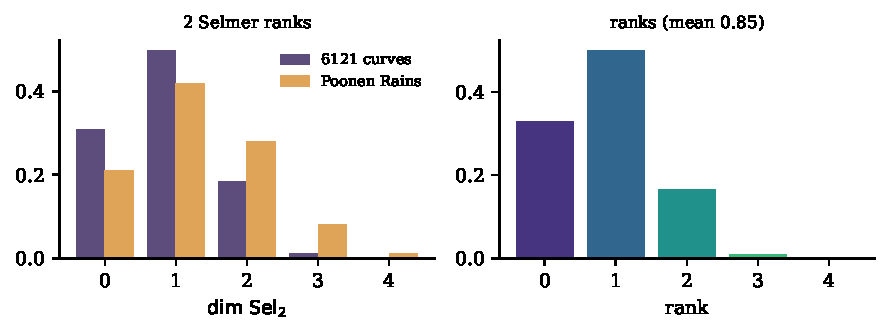
\includegraphics[width=0.92\textwidth]{figs/selmer_ranks.pdf}
\caption{Left: $\dim\operatorname{Sel}_2$ for the $6121$ curves of small height of Table~\ref{tab:06cselmer} against the Poonen Rains law. Right: their ranks (mean $0.85$).}\label{fig:06cselmer}
\end{figure}

Every frequency departs from the limiting law in the same direction: small Selmer groups are too common, and large ones too rare. The mean of $|\operatorname{Sel}_2|$ is $2.119$, not $3$. Yet the mean rank, $0.853$, is far above the conjectural limit $\frac12$, and one curve in six has rank $2$. The two effects are compatible. The mean of $\dim\operatorname{Sel}_2$ is $0.894$, only $0.041$ above the mean rank. For a curve whose rank the descent determines, $\dim\operatorname{Sel}_2-r = \dim\mathrm{Sha}(E)[2]$ is even (Section~\ref{sec:06cparity}), and here $\dim\operatorname{Sel}_2\le3$, so $\mathrm{Sha}(E)[2]\cong(\Z/2)^2$ for exactly $125$ curves ($2.0\%$) and $\mathrm{Sha}(E)[2] = 0$ for the rest: at small height, $\operatorname{Sel}_2$ is almost entirely accounted for by rational points. This is what the conjecture of Birch and Swinnerton Dyer leads one to expect, since together with standard conjectures on $L(E,1)$ it gives $|\mathrm{Sha}|$ an average size $H^{1/12+o(1)}$ over curves of rank $0$ \cite{ppvw2019}, which is small at our heights ($H\le256000$). In the model of Park, Poonen, Voight and Wood both features appear at small height: the cokernel that models $\mathrm{Sha}$ is small, and the probability of rank at least $2$ decays only like $H^{-1/24+o(1)}$. The excess of rank $2$ in small height families was documented systematically by Bektemirov, Mazur, Stein and Watkins \cite{bmsw2007}, who argued that the convergence to the limiting average is slow (a heuristic of Watkins discussed there makes the proportion of analytic rank at least $2$ among curves of root number $+1$ and discriminant near $X$ decay like $(\log X)^{3/8}X^{-1/24}$) and that the data do not contradict the minimalist conjecture. We read our table in the same cautious way: a box with $|a|,|b|\le40$ is far from the asymptotic regime. Section~\ref{sec:06cparity} examines the statistic that should already be close to its limit, the proportion of curves with root number $+1$.

\section{Ranks and $L$ functions}\label{sec:06cranks}

\subsection{Goldfeld's conjecture and the minimalist conjecture}

For a fixed $E/\Q$ of conductor $N_E$ and fundamental discriminants $d$, the quadratic twists $E_d$ have $L(s,E_d) = \sum\chi_d(n)a_nn^{-s}$ (away from the conductor), and for $d$ prime to $N_E$ the root number is $w(E_d) = \chi_d(-N_E)w(E)$, so these twists split evenly between root numbers $+1$ and $-1$.

\begin{conjecture}[Goldfeld \cite{goldfeld1979}]\label{conj:06cgoldfeld}
In the family of quadratic twists of a fixed elliptic curve over $\Q$, ordered by $|d|$, the average analytic rank is $\frac12$: asymptotically half the twists have analytic rank $0$ and half have analytic rank $1$.
\end{conjecture}

The minimalist conjecture is the analogous statement for all elliptic curves ordered by height, or for any reasonable family: the rank is as small as the root number allows, so rank $0$ when $w = +1$ and rank $1$ when $w = -1$, outside a set of density zero. Both are predictions of the Katz and Sarnak philosophy (Chapter~\ref{ch:06}): for a family with orthogonal symmetry split by root number, the zeros near the centre behave like eigenvalues near $1$ of Haar random matrices in $\mathrm{SO}(2N)$ or $\mathrm{SO}(2N+1)$, and a random matrix in $\mathrm{SO}(2N)$ has eigenvalue $1$ with probability $0$, while one in $\mathrm{SO}(2N+1)$ has it with multiplicity exactly $1$ almost surely. The random alternating matrices of the BKLPR model make the same prediction on the arithmetic side: kernel rank $0$ or $1$ according to the parity of $n$. That two random matrix models, one for zeros (orthogonal) and one for groups (alternating $p$ adic), agree on the $50/50$ split is an instance of the dictionary between the analytic and arithmetic sides of the conjecture of Birch and Swinnerton Dyer.\index{Goldfeld conjecture}\index{minimalist conjecture}

The rigorous results are bounds. Under the generalized Riemann hypothesis, the one level density methods of Brumer, Heath Brown and Young described in Section~\ref{sec:ch6ils} bound the average analytic rank; the Bhargava and Shankar theorems give unconditional bounds for the average algebraic rank. In quadratic twist families Smith \cite{smith2017} proved, in a preprint, that for $E/\Q$ with full rational $2$ torsion and no rational cyclic subgroup of order $4$ the $2^\infty$ Selmer groups of the twists $E_d$ have the distribution predicted by Delaunay's heuristic, and deduced that the twists of rank at least $2$ have density zero, the algebraic heart of Goldfeld's conjecture for these families.

\subsection{Root numbers and parity}\label{sec:06cparity}

Among the $6121$ curves of Table~\ref{tab:06cselmer} the root number is $+1$ for $49.2\%$, and for every one of them the rank is even exactly when $w(E) = +1$. This is what the parity conjecture $(-1)^{r(E)} = w(E)$ predicts; it follows from the conjecture of Birch and Swinnerton Dyer and is open in general. What is proved is the $p$ parity conjecture: Monsky \cite{monsky1996} showed that $(-1)^{\dim\operatorname{Sel}_2(E)-\dim E(\Q)[2]} = w(E)$ for every $E/\Q$, and T.~and V.~Dokchitser \cite{dokchitser2010} proved that the $\Z_p$ corank of the $p^\infty$ Selmer group has the parity of the root number for every $E/\Q$ and every prime $p$. Rank parity follows for every curve with $\mathrm{Sha}(E)[p^\infty]$ finite for one $p$, since that corank is then the rank. Our check is therefore not independent evidence for the parity conjecture. The upper bound that \texttt{ellrank} computes exceeds the rank by the dimension of $2\,\mathrm{Sha}(E)[4]$, so when the bounds coincide $\mathrm{Sha}(E)$ has no element of order $4$; then $\mathrm{Sha}(E)[2^\infty] = \mathrm{Sha}(E)[2]$ is finite, of even dimension, and Monsky's theorem forces the agreement. For the same reason the even parts of the two distributions, $0.3093+0.1826$ and $0.3277+0.1642$, both equal the root number proportion $0.4919$. What the data test is the equidistribution of root numbers, and $0.4919$ is within $1.3$ standard errors of $\frac12$.

\subsection{The rank as a Thorin atom and as a bias}

The rank enters the analytic theory of this book in two further guises. In Chapter~\ref{ch:05} we saw that the partial sums $\sum_{p\le x}a_p\log p/p$ drift like $(\frac12-r)\log x$ in logarithmic mean under the Riemann hypothesis for $L(s,E)$ (Section~\ref{sec:05bias}, Table~\ref{tab:05bias}): the central zero of order $r$ appears, through the explicit formula, as a bias in Frobenius traces. In Chapter~\ref{ch:10b} (Proposition~\ref{prop:10brank}) the same central zero appears as a degenerate Thorin atom: $\log|\Lambda(\frac12+\sqrt s,E)|$ has slope $r/2$ in $\log s$ near $s = 0$, a gamma factor of shape $r/2$ whose Thorin mass has escaped to the origin. In the language of the present chapter the minimalist conjecture, in its analytic form, says that in a family this atom has mass $0$ or $\frac12$ according to the root number, each with probability $\frac12$, and that the larger masses $1,\frac32,\dots$ occur with density zero. Our small height data, with mean rank $0.853$, put visible weight on the larger masses: by the theorems of Gross and Zagier \cite{grosszagier1986} and Kolyvagin \cite{kolyvagin1988} a curve of rank at least $2$ has analytic rank at least $2$, and $17.3\%$ of our curves have rank at least $2$. The rank bias and the Thorin atom read the order of vanishing at the centre directly; the Selmer statistics read it through the conjecture of Birch and Swinnerton Dyer.

\subsection{The Poonen Rains law as a sum of independent coins}

We close the mathematical part of the chapter with a structural description of the Poonen Rains law that makes its moments transparent.

\begin{proposition}[Poonen and Rains \cite{poonenrains2012}]\label{prop:06cbernoulli}
Let $\xi_0,\xi_1,\dots$ be independent with $\Prob(\xi_i = 1) = 1/(1+p^i) = 1-\Prob(\xi_i = 0)$. Then:
\begin{enumerate}[label=(\alph*)]
\item for each $n$, $\dim W\cap Z$ in Theorem~\ref{thm:06cpr} has the law of $\xi_0+\dots+\xi_{n-1}$, and the Poonen Rains law \eqref{eq:06cprlaw} is the law of $S = \sum_{i\ge0}\xi_i$, which is almost surely finite;
\item $\E t^S = \prod_{i\ge0}(t+p^i)/(1+p^i)$ for all complex $t$;
\item $\Prob(S\text{ even}) = \frac12$, and $S$ is even with probability $\frac12$ conditionally on $\xi_1,\xi_2,\dots$;
\item $\E p^S = p+1$, and more generally $\E\prod_{j=0}^{k-1}(p^S-p^j) = p^{k(k+1)/2}$ for $k\ge1$;
\item $\E S = \sum_{i\ge0}(1+p^i)^{-1}$ and $\operatorname{Var}S = \sum_{i\ge0}p^i(1+p^i)^{-2}$; for $p = 2$ these are $1.2645$ and $0.8463$;
\item $\Prob(S = 0) = c_p := \prod_{j\ge0}(1+p^{-j})^{-1}$ and $\Prob(S\ge2) = 1-\frac{2p-1}{p-1}\,c_p$, equal to $1-3c_2 = 0.3709$ for $p = 2$.
\end{enumerate}
\end{proposition}

\begin{proof}
(a) By Theorem~\ref{thm:06cpr} the generating function of $\dim W\cap Z$ is
\[
\begin{aligned}
\E t^{\dim W\cap Z} &= \frac{1}{\prod_{i<n}(1+p^i)}\sum_{d=0}^n\binom nd_{\!p}p^{(n-d)(n-d-1)/2}t^d\\
&= \frac{t^n}{\prod_{i<n}(1+p^i)}\sum_{e=0}^n\binom ne_{\!p}p^{e(e-1)/2}t^{-e},
\end{aligned}
\]
substituting $e = n-d$ and using $\binom nd_p = \binom n{n-d}_p$. The $q$ binomial theorem $\sum_e\binom ne_pp^{e(e-1)/2}u^e = \prod_{i<n}(1+p^iu)$ with $u = 1/t$ gives $\prod_{i<n}(t+p^i)/(1+p^i)$, the generating function of $\xi_0+\dots+\xi_{n-1}$, since $(t+p^i)/(1+p^i) = \Prob(\xi_i = 0)+t\Prob(\xi_i = 1)$. Since $\sum_i\Prob(\xi_i = 1)<\infty$, Borel and Cantelli show that only finitely many $\xi_i$ equal $1$, so the partial sums converge almost surely to $S<\infty$; hence the laws converge pointwise, and the limit is \eqref{eq:06cprlaw} by Theorem~\ref{thm:06cpr}. (b) The partial products converge for every $t$ because $\sum_i|t-1|/(1+p^i)<\infty$, and $\E t^{S_n}\to\E t^S$ by dominated convergence for $|t|\le1$ and, for larger $|t|$, by the bound $|t|^{S_n}\le|t|^S$ and the finiteness of $\E|t|^S = \prod_i(|t|+p^i)/(1+p^i)$ (monotone convergence). (c) $\xi_0$ is a fair coin independent of $\xi_1,\xi_2,\dots$, so the parity of $S$ is a fair coin given the rest. (d) Fix $W$ in $V_n$ and $k\le n$. A $k$ tuple of linearly independent vectors in $W\cap Z$ spans a $k$ dimensional subspace $U\subset W$, and, as in the proof of Theorem~\ref{thm:06cpr}, the maximal isotropic $Z$ containing a given $U$ correspond to the maximal isotropic subspaces of $U^\perp/U\cong V_{n-k}$, of which there are $\prod_{i<n-k}(1+p^i)$. Counting pairs,
\[
\E\prod_{j<k}\bigl(p^{\dim W\cap Z}-p^j\bigr) = \prod_{j<k}(p^n-p^j)\,\frac{\prod_{i<n-k}(1+p^i)}{\prod_{i<n}(1+p^i)} = \prod_{j<k}\frac{p^n-p^j}{1+p^{n-k+j}} ,
\]
which tends to $\prod_{j<k}p^{k-j} = p^{k(k+1)/2}$ as $n\to\infty$. By (a) the left side is $\E f(S_n)$ with $S_n = \xi_0+\dots+\xi_{n-1}$ and $f(m) = \prod_{j<k}(p^m-p^j)$, which is nonnegative and nondecreasing on the integers; since $S_n$ increases to $S$, monotone convergence gives $\E f(S) = p^{k(k+1)/2}$. The case $k = 1$ is $\E p^S = p+1$. (e) Sum the Bernoulli means and variances. (f) $\Prob(S = 0) = \prod_i\Prob(\xi_i = 0) = \prod_ip^i/(1+p^i)$, and $\Prob(S = 1) = \Prob(S = 0)\sum_i\Prob(\xi_i = 1)/\Prob(\xi_i = 0) = \Prob(S = 0)\sum_ip^{-i} = \Prob(S = 0)\,p/(p-1)$.
\end{proof}

Parts (a) and (b) are Proposition~2.6 of Poonen and Rains, (c) is their Proposition~2.22(b), and (d) is equivalent to their Proposition~2.22(a); in the form stated, (d) is the prime case of a theorem of Bhargava, Kane, Lenstra, Poonen and Rains \cite{bklpr2015}, proved there by the same count. The independent coin form separates parity from size. For a curve with $E(\Q)[p] = 0$ the theorem of Dokchitser and Dokchitser gives $(-1)^{\dim\operatorname{Sel}_p(E)} = w(E)$, because $\operatorname{Sel}_p(E) = \operatorname{Sel}_{p^\infty}(E)[p]$ and the quotient of $\operatorname{Sel}_{p^\infty}(E)$ by its divisible part, which carries the nondegenerate alternating Cassels Tate pairing, has $p$ torsion of even dimension. In the model the parity of $S$ plays the role of $w(E)$, and by (c) it is a fair coin even given $\xi_1,\xi_2,\dots$, as equidistributed root numbers require. In the BKLPR model the rank $r$ is $0$ or $1$ almost surely and $\dim\operatorname{Sel}_p = r+\dim\mathrm{Sha}[p]$ with $\dim\mathrm{Sha}[p]$ even, so $r$ is the parity of $S$ and $\dim\mathrm{Sha}[p] = 2\lfloor S/2\rfloor$; for $p = 2$ the coins $\xi_1,\xi_2,\dots$, with probabilities $\frac13,\frac15,\frac19,\dots$, govern its size.

\begin{corollary}[Rank bounds from the model]\label{cor:06cbound}
Consider a family of elliptic curves over $\Q$ with $E(\Q)[2] = 0$, ordered by a height, in which $\dim\operatorname{Sel}_2(E)$ converges in distribution to the Poonen Rains law \eqref{eq:06cprlaw} for $p = 2$ and the average of $|\operatorname{Sel}_2(E)|$ over the curves of height at most $X$ stays bounded as $X\to\infty$. Then the average rank $\bar r(X)$ of the curves of height at most $X$ satisfies
\[
\limsup_{X\to\infty}\bar r(X)\le\E S = \sum_{i\ge0}\frac{1}{1+2^i} = 1.2645 < \log_2\E2^S = \log_23 = 1.585 ,
\]
where $S$ has the law \eqref{eq:06cprlaw} for $p = 2$.
\end{corollary}

\begin{proof}
Since $E(\Q)[2] = 0$, the Kummer map embeds $E(\Q)/2E(\Q)\cong(\Z/2)^r$ in $\operatorname{Sel}_2(E)$, so $r\le\dim\operatorname{Sel}_2(E)$. For every $\varepsilon>0$ there is $C_\varepsilon$ with $m\le C_\varepsilon+\varepsilon2^m$ for all $m\ge0$, so bounded averages of $2^{\dim\operatorname{Sel}_2}$ make $\dim\operatorname{Sel}_2$ uniformly integrable along the family, and its averages converge to $\E S$, which Proposition~\ref{prop:06cbernoulli}(e) evaluates. The last comparison is Jensen's inequality for the concave logarithm, strict because $S$ is not constant, with $\E2^S = 3$ from Proposition~\ref{prop:06cbernoulli}(d).
\end{proof}

The comparison clarifies what an average of $|\operatorname{Sel}_2|$ alone can give. Knowing only that the average of $|\operatorname{Sel}_2|$ is $3$, as Bhargava and Shankar proved, Jensen yields average rank at most $\log_23\approx1.585$; the integer inequality $2r\le2^r$ does better and yields their bound $1.5$. Knowing in addition the full Poonen Rains law would give $1.2645$. The same argument with the integer inequalities $r\le\frac12+\frac16\,3^r$ and $r\le\frac34+\frac1{20}\,5^r$, both equalities at $r = 1,2$, turns the $3$ Selmer average $4$ into their bound $\frac76\approx1.17$ and the $5$ Selmer average $6$ into $1.05$, before the parity input described after Theorem~\ref{thm:06cbs}. The value $\frac12$ is out of reach of the Selmer group at any single prime, even with its full law: Selmer data alone cannot exclude $r = \dim\operatorname{Sel}_p$, so the best bound they give is $\E\dim\operatorname{Sel}_p = \sum_{i\ge0}(1+p^i)^{-1}$ in the model, which exceeds $\frac12$ for every $p$. It tends to $\frac12$ as $p\to\infty$, and Rubin observed \cite{poonenrains2012} that the law \eqref{eq:06cprlaw} itself tends to the fair coin on $\{0,1\}$. Hence the average rank would be at most $\frac12$ if Conjecture~\ref{conj:06cpr} and the average $p+1$ of $|\operatorname{Sel}_p|$, which Poonen and Rains also conjecture, held for infinitely many $p$. The law alone for infinitely many $p$ would give the density statements that almost all curves have rank at most $1$ and at least half have rank $0$, but not the bound on the average, since a set of curves of density zero and large rank could raise it.

\section{Notes}

Cohen and Lenstra \cite{cohenlenstra1984} introduced the heuristics in the Noordwijkerhout proceedings, with extensive tables; Cohen and Martinet \cite{cohenmartinet1990} extended them to general number fields. The random matrix interpretation is due to Friedman and Washington \cite{friedmanwashington1989}, in the function field setting, where the $\ell$ part of the class group is the cokernel of $1-\Frob$ acting on the $\ell$ adic Tate module of the Jacobian. Hall's identity \cite{hall1938} predates both. Wood developed the moment method \cite{wood2017} and showed \cite{wood2019} that cokernels of random integral matrices with quite general independent entries have Cohen Lenstra limits, a universality phenomenon analogous to the universality of eigenvalue statistics in Chapter~\ref{ch:06}. The sandpile groups of supersingular isogeny graphs, which are modules over a Hecke algebra $\mathbb T$, behave differently: for a fixed characteristic $N\equiv1\bmod12$, growing isogeny degree and all but finitely many primes $r$, their $r$ parts follow the law of $\mathbb T_r/\det(\gamma-1)\mathbb T_r$ for $\gamma$ Haar random in the subgroup of $\GL_2(\mathbb T_r)$ with determinant in $\Z_r^\times$, where $\mathbb T_r=\mathbb T\otimes\Z_r$, and this law is not the Cohen Lenstra law (Munier and Shnidman \cite{muniershnidman2023}; Chapter~\ref{ch:hit}).

The theorem of Davenport and Heilbronn \cite{davenportheilbronn1971} is still the only determination of the mean of $|\mathrm{Cl}(D)[p]|$ over quadratic fields for an odd prime $p$. Bhargava's higher composition laws and his count of quartic rings and fields \cite{bhargava2005} carried such averages beyond the quadratic case; the secondary term \cite{bst2013,taniguchithorne2013} confirmed Roberts's conjecture. The function field results \cite{evw2016} brought topology (homological stability of Hurwitz spaces) into arithmetic statistics. The corrections at roots of unity are in Malle \cite{malle2008}.

The Poonen Rains model \cite{poonenrains2012} was motivated in part by the earlier theorems of Heath Brown on $2$ Selmer groups in the congruent number family and of Swinnerton Dyer and Kane on quadratic twists of curves with full rational $2$ torsion and no rational cyclic subgroup of order $4$, which give the law \eqref{eq:06cprlaw} for $p = 2$, shifted by $2$ to account for $E[2]$, in these twist families. The theorems of Bhargava and Shankar \cite{bhargavashankar2015,bhargavashankar2015b,bhargavashankar2013} and the synthesis of \cite{bklpr2015} and \cite{ppvw2019} now frame the subject, and the database of Balakrishnan, Ho, Kaplan, Spicer, Stein and Weigandt \cite{bhkssw2016} tests these models on hundreds of millions of curves ordered by height. Bektemirov, Mazur, Stein and Watkins \cite{bmsw2007} discuss the tension between data and the minimalist conjecture. The proposal that the Langlands programme be read alongside random group models is not ours; it is implicit in the way the conjecture of Birch and Swinnerton Dyer connects automorphic $L$ functions to Selmer and Shafarevich Tate groups.

\section{Exercises}

\begin{enumerate}
\item (Hall's identity in small order.) List the abelian groups of order $p^2$ and $p^3$ with their automorphism groups, and verify that $\sum_{|G| = p^n}|\operatorname{Aut}G|^{-1}$ equals the coefficient of $x^n$ in $\prod_{k\ge1}(1-xp^{-k})^{-1}$ for $n = 1,2,3$. Deduce \eqref{eq:06chall} by setting $x = 1$, assuming the generating function identity.
\item (Rank $0$ over a finite field.) Show that the probability that a uniformly random $n\times n$ matrix over $\mathbb{F}_p$ is invertible is $\eta_n(p)$, that it decreases in $n$, and that $0\le\eta_n(p)-\eta_\infty(p)\le p^{-n}/(p-1)$. Compute $\eta_n(2)$ for $n = 1,\dots,5$ and compare with $\eta_\infty(2) = 0.2888$.
\item (Poonen Rains at $d = 0$.) Using Theorem~\ref{thm:06cpr}, show that $\Prob(\operatorname{Sel}_2 = 0)$ is predicted to be $\prod_{j\ge0}(1+2^{-j})^{-1} = 0.2097$, and that the finite $n$ value is $2^{n(n-1)/2}/\prod_{i<n}(1+2^i)$. Compute it for $n = 1,\dots,6$.
\item (The constant at $3$.) Compute $\eta_\infty(3)$ to six digits using Euler's pentagonal number theorem, $\eta_\infty(p) = \sum_{k\in\Z}(-1)^kp^{-k(3k-1)/2}$, and determine how many terms are needed for six digits. Deduce the Cohen Lenstra prediction $\Prob(3\mid h(D)) = 0.4399$.
\item (Mean of $|G[p]|$.) Let $\bar A$ be a uniformly random $n\times n$ or $n\times(n+1)$ matrix over $\mathbb{F}_p$. By summing $\Prob(\bar A^{\mathsf T}v = 0)$ over $v\in\mathbb{F}_p^n$, show that $\E|\ker\bar A^{\mathsf T}|$ equals $2-p^{-n}$ in the square case and $1+p^{-1}-p^{-n-1}$ in the rectangular case. Since $|G[p]| = p^{\operatorname{rk}_pG}$ and $p^{\operatorname{rk}_p\operatorname{cok}A} = |\ker\bar A^{\mathsf T}|$ when $\bar A$ is the reduction of $A$ modulo $p$, deduce $\E_{\mu_{\mathrm{CL}}}|G[p]| = 2$ and $\E_{\mu^+_{\mathrm{CL}}}|G[p]| = 1+p^{-1}$, justifying the passage to the limit as in the proof of Proposition~\ref{prop:06cmoments}. Compare with Theorem~\ref{thm:06cdh}.
\item (Parity.) In the setting of Proposition~\ref{prop:06cbernoulli}, show that $\E(-1)^S = 0$, by evaluating the generating function at $t = -1$, and that $\Prob(\dim W\cap Z\text{ even}) = \frac12$ for every finite $n\ge1$. Show that if root numbers in a family of curves without rational $2$ torsion are $+1$ and $-1$ with limiting proportions $\frac12(1+\beta)$ and $\frac12(1-\beta)$, then by Monsky's theorem $\dim\operatorname{Sel}_2$ cannot follow the Poonen Rains law unless $\beta = 0$. Check that our data, with $\beta = -0.016$, are consistent with $\beta = 0$ at the usual significance levels.
\end{enumerate}

\section{Open computational problems}

\begin{compproblem}[Cohen Lenstra at scale with the secondary term]\label{cp:06cclscale}
Objective: measure the convergence of $3$, $5$ and $7$ parts of class groups of quadratic fields to the Cohen Lenstra laws, separating the secondary term. Objects: fundamental discriminants $D$, imaginary and real, all those with $|D|\le10^9$ and all those in the windows $X-10^8<|D|\le X$ for $X = 10^{10}$ and $10^{11}$. Route: PARI/GP \texttt{quadclassunit} (conditional on the generalized Riemann hypothesis, as for our data) or the subexponential class group algorithms of Jacobson and collaborators, distributed over discriminant windows on a cluster; for $3$ torsion alone, count cubic fields with Belabas's program as an unconditional check. Deliverable: tables of $p$ rank frequencies and of the means of $|\mathrm{Cl}(D)[p]|$ per window; a weighted least squares fit of $c+c'X^{-1/6}+c''X^{-1/3}$ to the $3$ torsion means, with the fitted $c'$ compared with the constants of Bhargava, Shankar and Tsimerman and of Taniguchi and Thorne; analogous fits for $p = 5,7$ with a free exponent. Why it matters: Table~\ref{tab:06cprank} shows a $3$ deficit of the size of the secondary term; a free exponent fit for $p\ge5$ would give an empirical rate of convergence where no theorem is known.
\end{compproblem}

\begin{compproblem}[Selmer groups and ranks by height]\label{cp:06cheight}
Objective: test the Poonen Rains law and the boundedness heuristic of Park, Poonen, Voight and Wood on curves ordered by height. Objects: all curves $y^2 = x^3+Ax+B$ with naive height $H\le10^{10}$ (about $10^8$ curves), with the database of Balakrishnan, Ho, Kaplan, Spicer, Stein and Weigandt \cite{bhkssw2016} as a starting point. Route: $2$ descent by PARI/GP \texttt{ellrank} or Magma, $3$ Selmer groups by Magma where feasible, root numbers from local data, and analytic ranks by \texttt{lfun} for a random subsample, distributed over curves on a cluster. Deliverable: the distribution of $\dim\operatorname{Sel}_2$ and $\dim\operatorname{Sel}_3$ in height windows, the mean of $|\operatorname{Sel}_2|$ against $3$, the proportion of rank $\ge2$ as a function of $H$ with a fitted power law, and the tail counts of rank $\ge r$ against the exponents predicted by \cite{ppvw2019}. Why it matters: the excess of curves of rank at least $2$ in Table~\ref{tab:06cselmer} must decay if the minimalist conjecture holds, and its rate of decay is what separates slow convergence from a genuine bias.
\end{compproblem}

\begin{compproblem}[Shafarevich Tate groups against BKLPR]
Objective: compare the analytic orders of $\mathrm{Sha}$ with the alternating cokernel model of \cite{bklpr2015} and with Delaunay's distribution. Objects: all curves of conductor up to $5\cdot10^5$ in Cremona's tables and the LMFDB \cite{lmfdb}, plus quadratic twist families of $11a1$ and $37a1$ with $|d|\le10^7$. Route: the analytic order of $\mathrm{Sha}$ from the leading term of $L(s,E)$ via the conjecture of Birch and Swinnerton Dyer (PARI/GP \texttt{ellbsd} and \texttt{lfun}), checked against $2$, $3$ and $4$ descents in Magma. Deliverable: the empirical law of $\mathrm{Sha}[p^\infty]$ for $p = 2,3,5$ in conductor windows, the proportion of nontrivial $\mathrm{Sha}$ as a function of conductor, and a fit of the effective matrix size in the model of Park, Poonen, Voight and Wood as a function of the conductor. Why it matters: our data show $\mathrm{Sha}[2]$ nontrivial for only $2\%$ of small curves; tracking how this grows tests the calibration on which the boundedness heuristic rests.
\end{compproblem}

\begin{compproblem}[Class groups of cubic and quartic fields]
Objective: test the Cohen Martinet heuristics, with Malle's corrections at roots of unity, for class groups of cubic and quartic fields. Objects: all cubic fields with $|D|\le10^{9}$ (enumerated by Belabas's algorithm) and all quartic fields with $|D|\le10^{8}$ with Galois groups $D_4$, $A_4$, $S_4$ and $C_4$; class groups for primes $p\le7$, with separate treatment of fields containing $\mu_p$ or with Galois closure containing it. Route: PARI/GP \texttt{bnfinit} under GRH, with spot certification by \texttt{bnfcertify}; Bhargava's parametrisations to enumerate quartic fields. Deliverable: $p$ rank frequencies against Cohen Martinet, including the average of $|\mathrm{Cl}[2]|$ for cubic fields against Bhargava's $\frac54$ and $\frac32$, and a table of the discrepancies at roots of unity against Malle's proposed corrections. Why it matters: these are the class groups attached to $\GL_1$ over fields of degree $3$ and $4$, and the cases where the heuristics are known to need correction are precisely where the arithmetic constraints are subtle.
\end{compproblem}
